% questions.tex -- Module 7 (The Nature of Light) short-answer booklet, HSC Section II style.
% 20 questions, 90 marks: Topic 1 Q1-5 (22 marks), Topic 2 Q6-10 (23), Topic 3 Q11-15 (22),
% Marking guidelines and sample answers: answers.tex.
% Every number (and the Q3 curves): checks/m7-short-answer/numbers.py
% Build: TEXINPUTS=.: xelatex questions.tex (twice)
\documentclass[12pt]{article}
\usepackage{quiz}
\hypersetup{pdftitle={Short Answer Questions - Module 7 - The Nature of Light}}

\begin{document}
\quiztitle{Year 12 Physics}{Short Answer Questions - Module 7 - The Nature of Light}
\begin{center}
  20 questions \textperiodcentered\ 90 marks \textperiodcentered\ allow about 2 hours 40 minutes\\[2pt]
  Show all working. Use $c = \qty{3.00e8}{m.s^{-1}}$, $h = \qty{6.626e-34}{J.s}$,
  $e = \qty{1.602e-19}{C}$, $m_\mathrm{e} = \qty{9.109e-31}{kg}$, $m_\mathrm{p} = \qty{1.673e-27}{kg}$,\\
  $b = \qty{2.898e-3}{m.K}$, $\mu_0 = 4\pi \times 10^{-7}\,\si{N.A^{-2}}$,
  $\varepsilon_0 = \qty{8.854e-12}{C^2.N^{-1}.m^{-2}}$, $\qty{1}{eV} = \qty{1.602e-19}{J}$.
\end{center}

% =====================================================================
\firsttopictitle{Topic 1 - Electromagnetic Spectrum}

% ---- Q1 (Maxwell: EM waves and their speed)
\begin{saq}{4}
\qpartL{a}{2}{Describe the structure of an electromagnetic wave, according to Maxwell's theory. Include a
labelled diagram.\par\vspace{2mm}\framebox[\linewidth]{\rule{0pt}{40mm}}}{4}
\qpartL{b}{2}{Show that $\dfrac{1}{\sqrt{\mu_0\varepsilon_0}}$ is equal to the speed of light, and explain why
this result was important.}{5}
\end{saq}

% ---- Q2 (Fizeau's toothed wheel)
\Needspace{40\baselineskip}
\begin{saq}{5}
The diagram shows a simplified version of Fizeau's apparatus for measuring the speed of light.
\begin{center}
  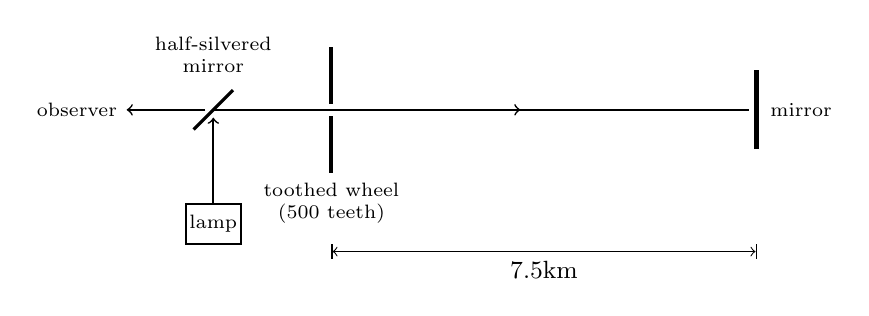
\begin{tikzpicture}
    \draw[line width=0.8pt] (1.45,-1.3) rectangle (2.15,-0.8); \node[font=\scriptsize] at (1.8,-1.05) {lamp};
    \draw[->, line width=0.6pt] (1.8,-0.8) -- (1.8,0.3);
    \draw[line width=1.2pt] (1.55,0.15) -- (2.05,0.65); \node[above, font=\scriptsize, align=center] at (1.8,0.75) {half-silvered\\mirror};
    \draw[line width=0.6pt] (1.8,0.4) -- (8.6,0.4);
    \draw[->, line width=0.6pt] (5.6,0.4) -- (5.7,0.4);
    \draw[->, line width=0.6pt] (1.7,0.4) -- (0.7,0.4); \node[left, font=\scriptsize] at (0.7,0.4) {observer};
    \draw[line width=1.4pt] (3.3,-0.4) -- (3.3,0.32); \draw[line width=1.4pt] (3.3,0.48) -- (3.3,1.2);
    \node[below, font=\scriptsize, align=center] at (3.3,-0.4) {toothed wheel\\(500 teeth)};
    \draw[line width=1.6pt] (8.7,-0.1) -- (8.7,0.9); \node[right, font=\scriptsize] at (8.75,0.4) {mirror};
    \draw[|<->|, line width=0.4pt] (3.3,-1.4) -- (8.7,-1.4) node[midway, below, font=\small] {\qty{7.5}{km}};
  \end{tikzpicture}
\end{center}
The wheel has 500 teeth, separated by gaps of the same width as the teeth. Light passes through a gap
between two teeth of the rotating wheel, travels \qty{7.5}{km} to a mirror and
returns along the same path. When the wheel turns slowly, the observer sees the returning light. As the
wheel speeds up, the light first disappears when the wheel turns at 20 revolutions per second, because the
returning light is blocked by the next tooth.
\qpartL{a}{2}{Explain why the light disappears at this speed of rotation.}{4}
\qpartL{b}{3}{Calculate the speed of light from these measurements.}{6}
\end{saq}

% ---- Q3 (black-body curves of two stars)
\Needspace{44\baselineskip}
\begin{saq}{5}
The graph shows the black-body radiation curves of two stars, X and Y, drawn to the same scale. The
spectrum of star X has its peak at \qty{414}{nm}. Star Y has a surface temperature of \qty{4500}{K}. The
shaded band shows the visible part of the spectrum.
\begin{center}
  \begin{tikzpicture}
    \fill[black!10] (1.6,0) rectangle (2.8,3.9); \node[font=\scriptsize] at (2.2,4.1) {visible};
    \draw[axisline] (0,0) -- (8.3,0) node[right, font=\small] {$\lambda$ (nm)};
    \draw[axisline] (0,0) -- (0,4.3) node[above, font=\small] {Intensity};
    \foreach \x/\l in {2/500, 4/1000, 6/1500, 8/2000} {\draw (\x,0) -- (\x,-0.08) node[below, font=\scriptsize] {\l};}
    \draw[line width=1pt, smooth] plot coordinates {(0.4,0.001) (0.5,0.015) (0.6,0.091) (0.7,0.300) (0.8,0.668) (0.9,1.163) (1.0,1.713) (1.1,2.247) (1.2,2.713) (1.3,3.083) (1.4,3.347) (1.5,3.512) (1.6,3.589) (1.7,3.594) (1.8,3.542) (1.9,3.448) (2.0,3.324) (2.1,3.179) (2.2,3.022) (2.3,2.859) (2.4,2.695) (2.5,2.533) (2.6,2.375) (2.7,2.223) (2.8,2.078) (2.9,1.941) (3.0,1.812) (3.1,1.691) (3.2,1.578) (3.3,1.473) (3.4,1.374) (3.5,1.283) (3.6,1.198) (3.7,1.119) (3.8,1.046) (3.9,0.979) (4.0,0.916) (4.1,0.857) (4.2,0.803) (4.3,0.753) (4.4,0.707) (4.5,0.664) (4.6,0.623) (4.7,0.586) (4.8,0.552) (4.9,0.519) (5.0,0.489) (5.1,0.461) (5.2,0.435) (5.3,0.411) (5.4,0.388) (5.5,0.367) (5.6,0.347) (5.7,0.329) (5.8,0.311) (5.9,0.295) (6.0,0.280) (6.1,0.265) (6.2,0.252) (6.3,0.239) (6.4,0.228) (6.5,0.217) (6.6,0.206) (6.7,0.196) (6.8,0.187) (6.9,0.178) (7.0,0.170) (7.1,0.162) (7.2,0.155) (7.3,0.148) (7.4,0.141) (7.5,0.135) (7.6,0.129) (7.7,0.124) (7.8,0.118) (7.9,0.113) (8.0,0.109)};
    \draw[line width=1pt, dash pattern=on 3pt off 2pt, smooth] plot coordinates {(0.4,0.000) (0.5,0.000) (0.6,0.000) (0.7,0.000) (0.8,0.002) (0.9,0.007) (1.0,0.018) (1.1,0.035) (1.2,0.060) (1.3,0.092) (1.4,0.128) (1.5,0.166) (1.6,0.205) (1.7,0.243) (1.8,0.277) (1.9,0.308) (2.0,0.333) (2.1,0.354) (2.2,0.371) (2.3,0.383) (2.4,0.390) (2.5,0.394) (2.6,0.395) (2.7,0.393) (2.8,0.389) (2.9,0.383) (3.0,0.375) (3.1,0.366) (3.2,0.356) (3.3,0.345) (3.4,0.334) (3.5,0.323) (3.6,0.311) (3.7,0.300) (3.8,0.288) (3.9,0.277) (4.0,0.266) (4.1,0.255) (4.2,0.244) (4.3,0.234) (4.4,0.224) (4.5,0.214) (4.6,0.205) (4.7,0.196) (4.8,0.188) (4.9,0.179) (5.0,0.172) (5.1,0.164) (5.2,0.157) (5.3,0.150) (5.4,0.144) (5.5,0.137) (5.6,0.132) (5.7,0.126) (5.8,0.121) (5.9,0.115) (6.0,0.111) (6.1,0.106) (6.2,0.101) (6.3,0.097) (6.4,0.093) (6.5,0.089) (6.6,0.086) (6.7,0.082) (6.8,0.079) (6.9,0.076) (7.0,0.073) (7.1,0.070) (7.2,0.067) (7.3,0.065) (7.4,0.062) (7.5,0.060) (7.6,0.057) (7.7,0.055) (7.8,0.053) (7.9,0.051) (8.0,0.049)};
    \draw[line width=1pt] (5.3,3.6) -- (6.0,3.6) node[right, font=\small] {Star X};
    \draw[line width=1pt, dash pattern=on 3pt off 2pt] (5.3,3.1) -- (6.0,3.1) node[right, font=\small] {Star Y};
  \end{tikzpicture}
\end{center}
\qpartL{a}{2}{Calculate the surface temperature of star X.}{4}
\qpartL{b}{2}{Star X looks white, but star Y looks orange-red. Explain this, with reference to the
graph.}{4}
\qpartL{c}{1}{Which star emits more energy from each square metre of its surface? Justify your answer
using the graph.}{2}
\end{saq}

% ---- Q4 (Doppler shift and line width)
\Needspace{40\baselineskip}
\begin{saq}{4}
The diagram compares the hydrogen absorption lines in the spectrum of a star with the same lines measured
in a laboratory. (The shift has been exaggerated so that it can be seen.)
\begin{center}
  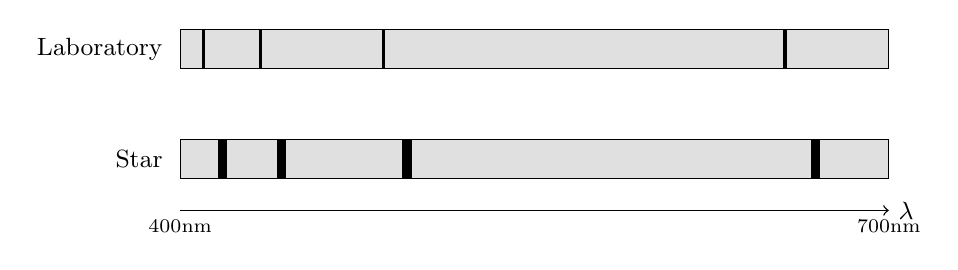
\begin{tikzpicture}
    \node[left, font=\small] at (-0.1,1.65) {Laboratory}; \node[left, font=\small] at (-0.1,0.25) {Star};
    \fill[black!12] (0,1.4) rectangle (9,1.9); \draw (0,1.4) rectangle (9,1.9);
    \fill[black!12] (0,0) rectangle (9,0.5); \draw (0,0) rectangle (9,0.5);
    \foreach \l in {410,434,486,656} {\pgfmathsetmacro\x{(\l-400)*0.03}\draw[line width=1.2pt] (\x,1.4) -- (\x,1.9);}
    \foreach \l in {418,443,496,669} {\pgfmathsetmacro\x{(\l-400)*0.03}\fill[black] (\x-0.06,0) rectangle (\x+0.06,0.5);}
    \draw[->, line width=0.5pt] (0,-0.4) -- (9,-0.4) node[right, font=\small] {$\lambda$};
    \node[below, font=\scriptsize] at (0,-0.4) {\qty{400}{nm}}; \node[below, font=\scriptsize] at (9,-0.4) {\qty{700}{nm}};
  \end{tikzpicture}
\end{center}
\qpartL{a}{2}{What can be concluded about the motion of the star? Justify your answer.}{4}
\qpartL{b}{2}{The lines in the star's spectrum are also broader than the laboratory lines. Give TWO
possible reasons for this.}{4}
\end{saq}

% ---- Q5 (chemical composition from spectra)
\Needspace{46\baselineskip}
\begin{saq}{4}
The diagram shows the absorption spectrum of a star, and the emission spectra of four elements measured in
a laboratory. All the spectra use the same wavelength scale.
\begin{center}
  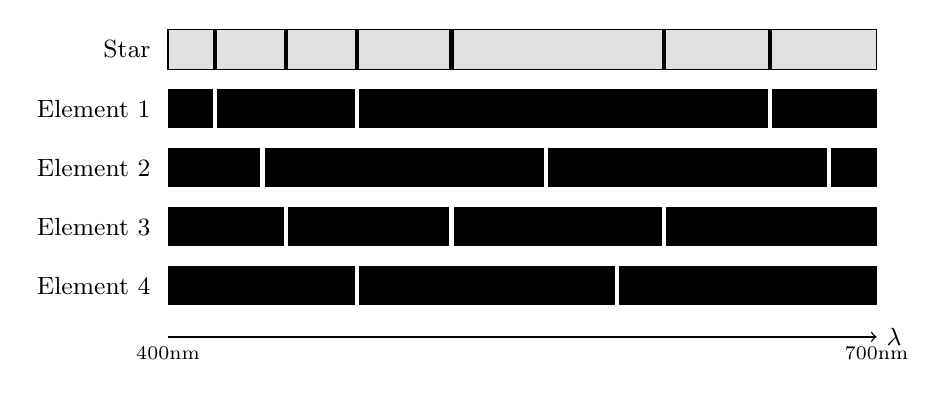
\begin{tikzpicture}
    \foreach \y/\l in {4/Star, 3/Element 1, 2/Element 2, 1/Element 3, 0/Element 4} {\node[left, font=\small] at (-0.1,\y*0.75+0.25) {\l};}
    \fill[black!12] (0,3) rectangle (9,3.5); \draw (0,3) rectangle (9,3.5);
    \foreach \l in {420,450,480,520,610,655} {\pgfmathsetmacro\x{(\l-400)*0.03}\draw[line width=1.5pt] (\x,3) -- (\x,3.5);}
    \foreach \y/\lines in {3/{420,480,655}, 2/{440,560,680}, 1/{450,520,610}, 0/{480,590}} {
      \pgfmathsetmacro\yy{\y*0.75}
      \fill[black] (0,\yy) rectangle (9,\yy+0.5);
      \foreach \l in \lines {\pgfmathsetmacro\x{(\l-400)*0.03}\draw[white, line width=1.5pt] (\x,\yy) -- (\x,\yy+0.5);}
    }
    \draw[->, line width=0.5pt] (0,-0.4) -- (9,-0.4) node[right, font=\small] {$\lambda$};
    \node[below, font=\scriptsize] at (0,-0.4) {\qty{400}{nm}}; \node[below, font=\scriptsize] at (9,-0.4) {\qty{700}{nm}};
  \end{tikzpicture}
\end{center}
\qpartL{a}{1}{Which of the four elements are present in the star's outer layers?}{2}
\qpartL{b}{3}{Explain how the dark lines in the star's spectrum are produced, and why they can be used to
identify the elements in the star.}{6}
\end{saq}

% =====================================================================
\topictitle{Topic 2 - Light: Wave Model}

% ---- Q6 (Young's double slit)
\begin{saq}{5}
Red laser light of wavelength \qty{633}{nm} shines on two narrow slits \qty{0.25}{mm} apart. An
interference pattern is seen on a screen \qty{3.0}{m} away.
\qpartL{a}{2}{Calculate the distance between neighbouring bright fringes on the screen.}{4}
\qpartL{b}{2}{Explain how the bright and dark fringes are formed.}{5}
\qpartL{c}{1}{Explain why this experiment supported the wave model of light rather than Newton's
particle model.}{3}
\end{saq}

% ---- Q7 (diffraction grating)
\Needspace{30\baselineskip}
\begin{saq}{5}
Light from a hydrogen lamp passes through a diffraction grating with 300 lines per millimetre.
\qpartL{a}{2}{Calculate the angle of the first-order maximum for the red hydrogen line,
$\lambda = \qty{656}{nm}$.}{4}
\qpartL{b}{2}{Another line has its first-order maximum at \ang{8.4}. Calculate its wavelength.}{4}
\qpartL{c}{1}{What is the highest order of the \qty{656}{nm} line that can be seen? Justify your
answer.}{2}
\end{saq}

% ---- Q8 (polarisation)
\Needspace{28\baselineskip}
\begin{saq}{4}
Unpolarised light of intensity \qty{60}{W.m^{-2}} passes through two polarising filters. The transmission
axis of the second filter is at \ang{30} to the axis of the first filter.
\qpartL{a}{1}{What is the intensity of the light after the first filter?}{2}
\qpartL{b}{1}{Calculate the intensity of the light after the second filter.}{3}
\qpartL{c}{2}{Explain how polarisation provides evidence about the nature of light.}{4}
\end{saq}

% ---- Q9 (Newton vs Huygens)
\Needspace{150mm}
\begin{saq}{5}
Compare Newton's particle model of light with Huygens' wave model, and assess how experimental evidence
was used to decide between them.
\alines{13}
\end{saq}

% ---- Q10 (investigation: wavelength of a laser)
\Needspace{125mm}
\begin{saq}{4}
Describe an investigation to measure the wavelength of light from a laser using a diffraction grating.
In your answer, include the measurements made, how the wavelength is calculated, and ONE way to improve
the accuracy of the result.
\alines{11}
\end{saq}

% =====================================================================
\topictitle{Topic 3 - Light: Quantum Model}

% ---- Q11 (black body, UV catastrophe, Planck)
\begin{saq}{4}
\qpartL{a}{1}{The surface temperature of the Sun is about \qty{5800}{K}. Calculate the wavelength at which
its emission is greatest.}{2}
\qpartL{b}{3}{Explain the difference between the classical prediction for black-body radiation and the
observed curves, and how Planck's hypothesis resolved this problem.}{7}
\end{saq}

% ---- Q12 (photoelectric calculation)
\Needspace{36\baselineskip}
\begin{saq}{5}
Light of wavelength \qty{400}{nm} shines on a potassium surface, which has a work function of
\qty{2.3}{eV}.
\qpartL{a}{1}{Calculate the energy of each photon, in electronvolts.}{3}
\qpartL{b}{1}{Calculate the maximum kinetic energy of the emitted photoelectrons, in joules.}{2}
\qpartL{c}{2}{Calculate the maximum speed of the photoelectrons.}{4}
\qpartL{d}{1}{What stopping voltage is needed to stop all the photoelectrons?}{2}
\end{saq}

% ---- Q13 (Kmax against f graph)
\Needspace{48\baselineskip}
\begin{saq}{5}
In a photoelectric experiment, a student measured the maximum kinetic energy $K_\mathrm{max}$ of the
photoelectrons emitted from a metal, for light of different frequencies $f$. The results are graphed below.
\begin{center}
  \begin{tikzpicture}[x=0.6cm, y=1.0cm]
    \draw[black!20, line width=0.3pt, xstep=0.5, ystep=0.5] (0,0) grid (12,4);
    \draw[axisline] (0,0) -- (12.6,0) node[right, font=\small, align=left] {$f$\\($\times10^{14}$ Hz)};
    \draw[axisline] (0,0) -- (0,4.5) node[above, font=\small] {$K_\mathrm{max}$ ($\times10^{-19}$ J)};
    \foreach \x in {0,2,...,12} \node[below, font=\scriptsize] at (\x,0) {\x};
    \foreach \y in {1,2,3,4} \node[left, font=\scriptsize] at (0,\y) {\y};
    \draw[line width=1pt] (5.5,0) -- (11.5,4.0);
    \foreach \x/\y in {6/0.333, 7/1.0, 8/1.667, 9/2.333, 10/3.0} \fill (\x,\y) circle (2.2pt);
  \end{tikzpicture}
\end{center}
\qpartL{a}{2}{Use the graph to determine a value for Planck's constant.}{4}
\qpartL{b}{2}{Determine the work function of the metal, in electronvolts.}{4}
\qpartL{c}{1}{Describe how the graph would be different for a metal with a larger work function.}{2}
\end{saq}

% ---- Q14 (Einstein vs the wave model)
\Needspace{120mm}
\begin{saq}{4}
Explain how Einstein's model of light accounts for TWO observations of the photoelectric effect that the
wave model of light could not explain.
\alines{11}
\end{saq}

% ---- Q15 (photons from a laser and a lamp)
\Needspace{34\baselineskip}
\begin{saq}{4}
A green laser emits \qty{2.0}{mW} of light of wavelength \qty{532}{nm}.
\qpartL{a}{1}{Calculate the energy of one photon of this light.}{2}
\qpartL{b}{1}{Calculate the number of photons the laser emits each second.}{2}
\qpartL{c}{2}{The laser releases electrons from a metal with a work function of \qty{2.0}{eV}. A
\qty{100}{W} infrared lamp, emitting light of wavelength \qty{1200}{nm}, releases no electrons from the
same metal. Explain why, using calculations.}{5}
\end{saq}

% =====================================================================
\topictitle{Topic 4 - Light and Special Relativity}

% ---- Q16 (light clock)
\begin{saq}{4}
A light clock is made of two parallel mirrors. A pulse of light bounces between them, and each round
trip is one \emph{tick}. The diagrams show the path of the light during one tick, as seen by an observer
moving with the clock (left) and by an observer who sees the clock move to the right at speed $v$ (right).
\begin{center}
  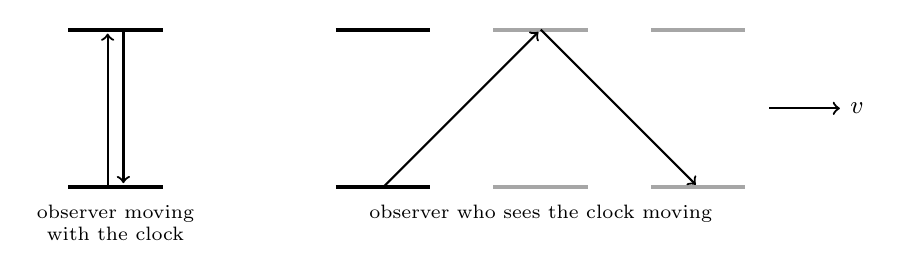
\begin{tikzpicture}
    \draw[line width=1.4pt] (0,0) -- (1.2,0); \draw[line width=1.4pt] (0,2) -- (1.2,2);
    \draw[->, line width=0.8pt] (0.5,0) -- (0.5,1.95); \draw[->, line width=0.8pt] (0.7,2) -- (0.7,0.05);
    \node[below, font=\scriptsize, align=center] at (0.6,-0.1) {observer moving\\with the clock};
    \foreach \x in {4,6,8} {\draw[line width=1.4pt, black!35] (\x-0.6,0) -- (\x+0.6,0); \draw[line width=1.4pt, black!35] (\x-0.6,2) -- (\x+0.6,2);}
    \draw[line width=1.4pt] (3.4,0) -- (4.6,0); \draw[line width=1.4pt] (3.4,2) -- (4.6,2);
    \draw[->, line width=0.8pt] (4,0) -- (5.97,1.97); \draw[->, line width=0.8pt] (6,2) -- (7.97,0.03);
    \draw[->, line width=0.8pt] (8.9,1.0) -- (9.8,1.0) node[right, font=\small] {$v$};
    \node[below, font=\scriptsize, align=center] at (6,-0.1) {observer who sees the clock moving};
  \end{tikzpicture}
\end{center}
Use the diagrams and Einstein's postulates to explain why the observer who sees the clock moving
measures a longer time for each tick than the observer moving with the clock.
\alines{9}
\end{saq}

% ---- Q17 (muons)
\Needspace{44\baselineskip}
\begin{saq}{5}
Muons are made when cosmic rays hit the upper atmosphere, \qty{10}{km} above Earth's surface. They travel
towards the ground at $0.998c$. At rest, muons have a mean lifetime of \qty{2.2}{\micro s}.
\qpartL{a}{1}{Calculate the distance a muon would travel in \qty{2.2}{\micro s}, ignoring
relativity.}{2}
\qpartL{b}{2}{Calculate the mean lifetime of the muons as measured by an observer on Earth, and the
distance they travel in this time.}{4}
\qpartL{c}{1}{Calculate the thickness of the \qty{10}{km} layer of atmosphere in the muons' frame of
reference.}{2}
\qpartL{d}{1}{Many muons are detected at Earth's surface. Explain how this supports special relativity.}{3}
\end{saq}

% ---- Q18 (trip to a star)
\Needspace{38\baselineskip}
\begin{saq}{5}
A spaceship travels from Earth to a star \num{4.2} light-years away (as measured from Earth), at a
constant speed of $0.80c$.
\qpartL{a}{1}{How long does the trip take, as measured by observers on Earth?}{2}
\qpartL{b}{2}{Calculate how long the trip takes, as measured by the astronauts.}{4}
\qpartL{c}{1}{Calculate the distance from Earth to the star, as measured by the astronauts.}{2}
\qpartL{d}{1}{Show that your answers to (b) and (c) are consistent with each other.}{2}
\end{saq}

% ---- Q19 (relativistic momentum and rest energy)
\Needspace{34\baselineskip}
\begin{saq}{5}
In a particle accelerator, a proton is accelerated to $0.95c$.
\qpartL{a}{2}{Calculate the relativistic momentum of the proton.}{4}
\qpartL{b}{1}{Calculate the rest energy of the proton, in joules.}{2}
\qpartL{c}{2}{Explain why the proton can never be accelerated to the speed of light, however much
energy is supplied.}{4}
\end{saq}

% ---- Q20 (aether, Michelson-Morley, postulates)
\Needspace{120mm}
\begin{saq}{4}
Explain how the result of the Michelson--Morley experiment and Einstein's postulates changed scientists'
ideas about the aether and the speed of light.
\alines{11}
\end{saq}

\end{document}
